\documentclass[titlepage,11pt]{article}
\usepackage{comment}
\usepackage{enumitem}
\usepackage{transparent} % Untuk transparansi gambar
\usepackage{listings}
\usepackage{amsmath}
\usepackage{graphicx}
\usepackage[font=small,labelfont=bf]{caption}
\usepackage[bahasa]{babel}
\usepackage{float}
\usepackage{verbatim}
\usepackage{graphicx,tabularx,multirow}
\usepackage{xcolor}
\usepackage[onehalfspacing]{setspace}
\usepackage[
	allcolors=visigrey,
	colorlinks=true,
]{hyperref}
\usepackage[a4paper,left=2cm,right=2cm]{geometry}
% Pengaturan kutipan artikel
\usepackage[style=ieee, backend=biber]{biblatex}
%Code listing style pak akok
\definecolor{codegreen}{rgb}{0,0.6,0}
\definecolor{codegray}{rgb}{0.5,0.5,0.5}
\definecolor{codepurple}{rgb}{0.58,0,0.82}
\definecolor{backcolour}{rgb}{0.95,0.95,0.92}

\usepackage{eso-pic} % Untuk menambahkan elemen ke seluruh halaman

\newcommand\BackgroundPic{
  \put(0,0){
    \parbox[b][\paperheight]{\paperwidth}{
      \vfill
      \centering
      \transparent{0.1}
      \includegraphics[width=0.4\paperwidth,keepaspectratio]{miot.png}
      \vfill
    }
  }
}

\newcommand\BackgroundAllPages{ \AddToShipoutPicture*{\BackgroundPic} }
\newcommand\BackgroundNone{ \ClearShipoutPicture } % hilangkan background

\lstdefinestyle{mystyle}{
	backgroundcolor=\color{backcolour}, commentstyle=\color{codegreen},
	keywordstyle=\color{magenta},
	numberstyle=\small\color{codegray},
	stringstyle=\color{codepurple},
	basicstyle=\ttfamily\footnotesize,
	breakatwhitespace=false,         
	breaklines=true,                 
	captionpos=t,                    
	keepspaces=true,                 
	numbers=left,                    
	numbersep=5pt,                  
	showspaces=false,                
	showstringspaces=false,
	showtabs=false,           
	frame = single,
	tabsize=2
}
\lstset{style=mystyle}

\definecolor{visigrey}{rgb}{.1,.15,.15}
\geometry{top=1cm,bottom=.5cm}
\savegeometry{titlepage}
\geometry{top=2cm,bottom=2cm}
\savegeometry{main}

\def\bspace{\(\qquad\qquad\qquad\)}
\usepackage[T1]{fontenc}
\usepackage[utf8]{inputenc}
\usepackage{tgheros}
\renewcommand*\familydefault{\sfdefault}

\setcounter{tocdepth}{6}

\def\autor{Laboratorium }
\def\lab{Multimedia dan Internet of Things}
\def\departemen{Departemen Teknik Komputer}
\def\institut{Institut Teknologi Sepuluh Nopember}
\def\praktikum{Laporan Akhir \\ Praktikum Jaringan Komputer}
\def\nama{Abraham Napitupulu - 5024231048}
% Ubah Judul sesuai dengan modul
\def\judul{Manajemen dan Routing IPv6}
\def\tanggal{2025}
\begin{document}
% Ubah Bahasa sesuai dengan keinginan
\selectlanguage{bahasa}

\BackgroundNone
\def\headingtype{\bf \small}
\loadgeometry{titlepage}

\begin{titlepage}
	\centering
	\begin{tabularx}{\textwidth}{l@{\hskip 0pt}lX}
		\raisebox{-0.5\height}{
\includegraphics[width=3cm]{Cover/img/logodepart.png}} 
		& \raisebox{-0.5\height}{\includegraphics[width=3cm]{Cover/img/miot.png}} 
		& \raggedleft
	\hfill
	\begin{minipage}{0.5\textwidth}
		\raggedleft
		{\emph{\headingtype \autor}} \\[-2pt]
		{\headingtype \lab} \\[-2pt]
		{\headingtype \departemen} \\[-2pt]
		{\headingtype \emph{\institut}}
	\end{minipage}

	\vspace{5cm}
	\end{tabularx}
	
	\vspace{5cm}
	{\Huge \bf \praktikum \par}
	
	\vspace{2cm}
	{\LARGE \bf \judul \par}
	
	\vspace{2cm}
	{\Large \nama \par}
	
	\vfill
	{\Large \tanggal \par}
	
	\vfill
	
\includegraphics[width=\textwidth]{Cover/img/footer.png}
\end{titlepage}

\loadgeometry{main}


\BackgroundAllPages
% Pilih Modul yang akan di build
\section{Pendahuluan}
\subsection{Latar Belakang}
IPv6 (Internet Protocol version 6) merupakan generasi terbaru dari sistem alamat internet yang dirancang untuk menggantikan IPv4. Dengan kapasitas alamat yang jauh lebih besar, IPv6 menyediakan sekitar 340 undecillion alamat unik, yang jauh melampaui batas 4,29 miliar alamat yang ditawarkan oleh IPv4. Teknologi ini muncul sebagai solusi untuk mengatasi kekurangan alamat IP yang terjadi akibat pesatnya pertumbuhan perangkat yang terhubung ke internet, termasuk Internet of Things (IoT) dan perangkat lainnya. IPv6 tidak hanya menawarkan jumlah alamat yang tak terbatas, tetapi juga fitur tambahan seperti keamanan yang lebih kuat dengan dukungan IPsec dan kemudahan konfigurasi otomatis melalui Stateless Address Auto Configuration (SLAAC). Meskipun demikian, transisi ke IPv6 memerlukan penyesuaian infrastruktur jaringan, karena belum semua perangkat dan sistem mendukung teknologi ini sepenuhnya. Router IPv6 memainkan peran kunci dalam penerapan teknologi ini, dengan memungkinkan pengelolaan alamat IP yang lebih efisien melalui konfigurasi statis atau dinamis, serta meningkatkan kecepatan dan keamanan jaringan secara keseluruhan.

\subsection{Dasar Teori}
IPv6 berfokus pada solusi untuk mengatasi keterbatasan alamat IP yang ada pada IPv4, yang hanya dapat menyediakan sekitar 4,29 miliar alamat. Dengan menggunakan sistem alamat 128-bit, IPv6 dapat menyediakan hingga 3,4 × 10³⁸ alamat unik, mengatasi kelangkaan alamat yang semakin meningkat seiring dengan berkembangnya perangkat yang terhubung ke internet. Selain itu, IPv6 menawarkan kemudahan konfigurasi otomatis melalui Stateless Address Auto Configuration (SLAAC) dan meningkatkan keamanan jaringan dengan dukungan IPsec dan fitur Secure Neighbor Discovery (SEND). Dengan menghilangkan kebutuhan akan Network Address Translation (NAT), IPv6 memungkinkan pengelolaan alamat yang lebih efisien dan jaringan yang lebih cepat serta aman. 

IPv4, yang menggunakan sistem alamat 32-bit, hanya dapat menyediakan sekitar 4,29 miliar alamat unik, sementara jumlah perangkat yang terhubung terus berkembang, termasuk perangkat-perangkat Internet of Things (IoT). Kekurangan alamat IP ini menjadi masalah utama, karena banyaknya perangkat yang memerlukan alamat IP untuk terhubung ke jaringan global. Untuk itu, IPv6 hadir dengan sistem alamat 128-bit yang mampu menyediakan 3,4 × 10³⁸ alamat, mengatasi masalah kelangkaan alamat IP secara signifikan.

Selain itu, IPv6 dirancang dengan mempertimbangkan kemudahan konfigurasi dan keamanan yang lebih baik dibandingkan dengan IPv4. Protokol ini mendukung Stateless Address Auto Configuration (SLAAC), yang memungkinkan perangkat untuk mengonfigurasi alamat IP secara otomatis tanpa bergantung pada server DHCP. Fitur ini meningkatkan efisiensi dalam pengelolaan jaringan, terutama pada jaringan besar dengan banyak perangkat.

IPv6 juga memperkenalkan penghapusan Network Address Translation (NAT), yang biasa digunakan pada IPv4 untuk mengatasi kekurangan alamat, namun sering menambah kompleksitas dan menurunkan kinerja jaringan. Keamanan juga menjadi fokus penting dalam IPv6, dengan dukungan terhadap IPsec untuk enkripsi dan otentikasi data secara end-to-end, serta fitur Secure Neighbor Discovery (SEND) untuk mencegah serangan terhadap perangkat jaringan.

\section{Tugas Pendahuluan}
\begin{enumerate}
    \item IPv6 menggunakan sistem alamat 128-bit, yang memungkinkan jumlah alamat yang hampir tak terbatas, sekitar 3,4 x 10³⁸ alamat. Hal ini mengatasi keterbatasan jumlah alamat pada IPv4, yang hanya menggunakan 32-bit dan menyediakan sekitar 4,29 miliar alamat.\\
    Perbedaan utama antara IPv6 dan IPv4 terletak pada panjang alamat, format penulisan, dan kapasitas alamat yang tersedia. IPv6 menggunakan alamat heksadesimal yang lebih panjang, sementara IPv4 menggunakan alamat desimal yang lebih pendek. IPv6 juga mendukung konfigurasi otomatis melalui Stateless Address Auto Configuration (SLAAC), sedangkan IPv4 bergantung pada DHCP (Dynamic Host Configuration Protocol) untuk konfigurasi alamat.\\
    Selain itu, IPv6 dilengkapi dengan fitur keamanan yang lebih baik, seperti dukungan IPsec untuk enkripsi dan autentikasi data, yang tidak tersedia secara default di IPv4. IPv6 juga tidak memerlukan Network Address Translation (NAT), yang sering digunakan pada IPv4 untuk mengatasi kekurangan alamat, sehingga meningkatkan efisiensi dan kecepatan jaringan.

    \item 
    \textbf{Alamat Asli:}
    Alamat IPv6 yang diberikan adalah 2001:db8::/32. Prefix ini menunjukkan bahwa bagian pertama dari alamat (32 bit pertama) digunakan untuk identifikasi jaringan utama. Sisa dari alamat (96 bit) dapat digunakan untuk subnet dan alamat host.

    \textbf{Pembagian menjadi empat subnet:}
    Untuk membagi menjadi empat subnet, kita membutuhkan dua bit tambahan pada bagian subnet. Hal ini karena dengan dua bit, kita bisa memiliki 4 kombinasi (2² = 4).

    \textbf{Prefix yang akan digunakan:}
    Dengan menambahkan dua bit, prefix baru yang digunakan akan menjadi /34 untuk bagian pertama subnet, dan selanjutnya kita akan memiliki /64 untuk masing-masing subnet.

    \textbf{Pembagian dan Alokasi Subnet IPv6:}
    \begin{itemize}
        \item Subnet A: \texttt{2001:db8:0000:0000::/64}
        \item Subnet B: \texttt{2001:db8:4000:0000::/64}
        \item Subnet C: \texttt{2001:db8:8000:0000::/64}
        \item Subnet D: \texttt{2001:db8:c000:0000::/64}
    \end{itemize}

    \item 
    \textbf{Alamat IPv6 pada masing-masing interface:}
    \begin{itemize}
        \item ether1 (Subnet A): \texttt{2001:db8:0000:0000::1/64}, Subnet: \texttt{2001:db8:0000:0000::/64}
        \item ether2 (Subnet B): \texttt{2001:db8:4000:0000::1/64}, Subnet: \texttt{2001:db8:4000:0000::/64}
        \item ether3 (Subnet C): \texttt{2001:db8:8000:0000::1/64}, Subnet: \texttt{2001:db8:8000:0000::/64}
        \item ether4 (Subnet D): \texttt{2001:db8:c000:0000::1/64}, Subnet: \texttt{2001:db8:c000:0000::/64}
    \end{itemize}

    \item 
    \textbf{Konfigurasi pada interface ethernet:}
    \begin{verbatim}
    set ether1 address=2001:db8:0000:0000::1/64
    set ether2 address=2001:db8:4000:0000::1/64
    set ether3 address=2001:db8:8000:0000::1/64
    set ether4 address=2001:db8:c000:0000::1/64
    \end{verbatim}

    \item 
    \textbf{Tabel Alamat IPv6 pada Subnet dan PC:}
    \begin{tabular}{|l|l|l|l|l|}
        \hline
        \textbf{Subnet} & \textbf{Prefix} & \textbf{Router IP (Interface)} & \textbf{PC1 IP} & \textbf{PC2 IP} \\
        \hline
        Subnet A & \texttt{2001:db8:0000:0000::/64} & \texttt{2001:db8:0000:0000::1} (ether1) & \texttt{2001:db8:0000:0000::10} & \texttt{2001:db8:0000:0000::11} \\
        Subnet B & \texttt{2001:db8:4000:0000::/64} & \texttt{2001:db8:4000:0000::1} (ether2) & \texttt{2001:db8:4000:0000::10} & \texttt{2001:db8:4000:0000::11} \\
        Subnet C & \texttt{2001:db8:8000:0000::/64} & \texttt{2001:db8:8000:0000::1} (ether3) & \texttt{2001:db8:8000:0000::10} & \texttt{2001:db8:8000:0000::11} \\
        Subnet D & \texttt{2001:db8:c000:0000::/64} & \texttt{2001:db8:c000:0000::1} (ether4) & \texttt{2001:db8:c000:0000::10} & \texttt{2001:db8:c000:0000::11} \\
        \hline
    \end{tabular}

    \item Routing statis pada jaringan IPv6 berfungsi untuk mengonfigurasi jalur rute secara manual, memberikan kontrol penuh kepada administrator untuk menentukan jalur yang akan dilalui paket data. Ini sangat berguna dalam jaringan kecil atau yang memiliki topologi tetap, di mana rute jarang berubah. Keuntungannya termasuk kestabilan jaringan yang lebih tinggi, karena rute tidak berubah kecuali ada intervensi manual, serta pengurangan overhead karena tidak memerlukan protokol routing dinamis. Routing statis lebih efisien pada jaringan yang sederhana, kecil, atau dengan sedikit perangkat, dan memberikan kontrol lebih ketat terhadap jalur data yang dilalui.\\
    Namun, untuk jaringan yang lebih besar atau dinamis, di mana perubahan topologi sering terjadi, routing dinamis lebih disarankan karena dapat menyesuaikan rute secara otomatis tanpa intervensi manual.
\end{enumerate}



\end{document}
